\chapter{Introducción}
\label{chap:antecedentes}

Los programas de computador comerciales para el análisis y diseño de estructuras que se encuentran vigentes a la fecha cuentan, en general, con un entorno gráfico que le permiten al usuario describir el modelo de forma interactiva, procesarlo y visualizar los resultados de manera conveniente.\\

En \cite{escamilla1995microcomputadores} se presenta una lista de algunos de estos programas de uso común en América Latina, entre los cuales se encuentra \emph{ETABS} (Three Dimensional Analysis of Building Systems - Extended Version).\\

ETABS es un programa de computador creado por Edward Wilson, Jeffery Hollings y Henry Dovey en 1975. Según \cite{ETABS1975}, este programa de computador fue desarrollado para el análisis estructural lineal de edificios de pórticos y muros a cortante sujetos tanto a cargas estáticas como sísmicas. El edificio es idealizado como un sistema de elementos tipo pórticos y muros a cortante independientes interconectado por losas de entrepiso las cuales son rígidas en su propio plano. \\

Este programa es una extensión de \emph{TABS} (Three Dimensional Analysis of  Building Systems) para permitir analizar pórticos en tres dimensiones. Según \cite{ETABS1972}, una de las razones para desarrollar este programa fue darle una retroalimentación a los usuarios de cuatro programas diferentes, \emph{FRMSTC}, \emph{FRMDYN}, \emph{LATERAL} y \emph{SAP}, que se usaban en varias estructuras importantes en diferentes países.\\

Estos programas, desarrollados en la Universidad de California, Berkeley, permitian el análisis lineal de edificios de varios pisos. FRMSTC (\emph{Static Load Analysis of High-Rise Buildings}) permitia analizar edificios simetricos con pórticos y muros a cortante paralelos sujetos a cargas estáticas. Las formas de los modos y las frecuencias también eran evaluadas. FRMDYN (\emph{Dynamic Analysis of Multistory Buildings}) era el mismo que FRMSTC con la excepción que la carga era la aceleración del terreno debido a un desplazamiento dependiente del tiempo. LATERAL fue una extensión de FRMSTC que permitia analizar linealmente pórticos y muros a cortante que no eran necesariamente paralelos. Habían tres grados de libertad en cada piso. Este programa no tenía la opción de realizar análisis dinámico. SAP (\emph{Structural Analysis Program}) era un programa general para el análisis de vigas complejas y de elementos finitos y tenía una opción que permitía introducir la aproximación de piso rígido. Este programa también tenía la opción de análisis dinámico. \\

En la actualidad, ETABS se encuentra en su versión 18.1.1 

Para usarlo, el usuario debe definir las características de la estructura mediante una serie de menús, como se muestra en la figura \ref{fig:sap2000_toolbar}. El programa permite establecer tipos de materiales, secciones transversales de los elementos, patrones de carga, entre otras características.

% % \textsuperscript{\textregistered}, 

\begin{figure}[ht]
    \centering
    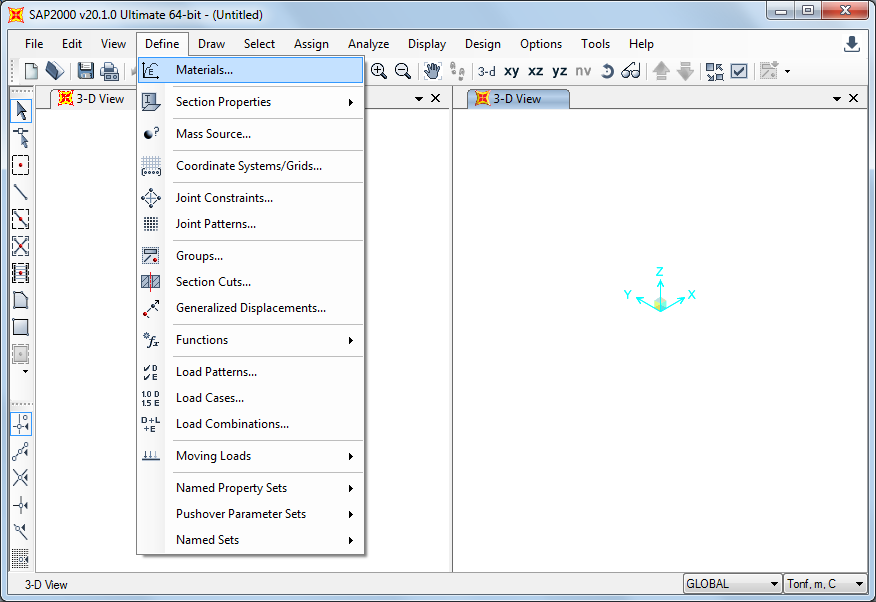
\includegraphics[width=1\textwidth]{metodologia/sap2000_toolbar.png}
    \caption{Menús del programa de computador SAP2000\textsuperscript{\textregistered} para definir las características de la estructura.}
    \label{fig:sap2000_toolbar}
\end{figure}

% % Dado que la intención de este trabajo es desarrollar un programa de computador a código abierto que cuente con características similares a los programas comerciales, en este capítulo se inicia identificando dichas características. Así mismo, se estudian las características de los programas a código abierto. \\

% % \section{Revisión de los programas comerciales}
% % La intensión de este trabajo fue realizar un programa de computador llamado \textit{StressUN} similar a los programas comerciales, de tal manera que se procedió a estudiar los diferentes elementos que los caracterizan. \\

% Una vez definidas las características de la estructura, el usuario procede a ingresar los diferentes elementos del modelo de la estructura en el entorno virtual de manera interactiva, mediante la ayuda de una serie de ejes y de los menús del programa. \\

% El entorno virtual consiste en un ambiente tridimensional donde el usuario puede ver, ingresar e interactuar con los diferentes elementos visuales del modelo.\\

% La serie de ejes consiste en un grupo de líneas en el espacio que se interceptan en un conjunto de puntos, los cuales sirven de referencia para que el usuario pueda ingresar los diferentes elementos del modelo al entorno virtual. En la figura \ref{fig:sap2000_axes} se presenta un conjunto de dichos ejes en el entorno virtual.\\
% \begin{figure}[ht]
%     \centering
%     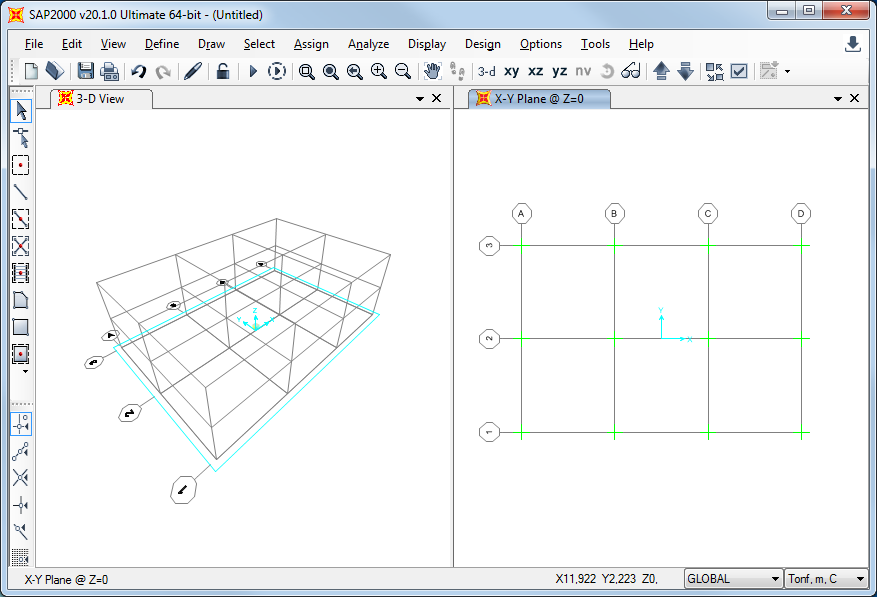
\includegraphics[width=1\textwidth]{metodologia/sap2000_axes.png}
%     \caption{Entorno virtual de SAP2000\textsuperscript{\textregistered} con un conjunto de ejes definido.}
%     \label{fig:sap2000_axes}
% \end{figure}

% Los menús del programa de computador que permiten ingresar los elementos del modelo consisten en aquellos que permiten escoger el tipo de elemento, como se muestra en la figura \ref{fig:sap200_draw}, y aquellos que permiten modificar los elementos ya ingresados, los cuales permiten moverlos, copiarlos, o eliminarlos. \\
% \begin{figure}[ht]
%     \centering
%     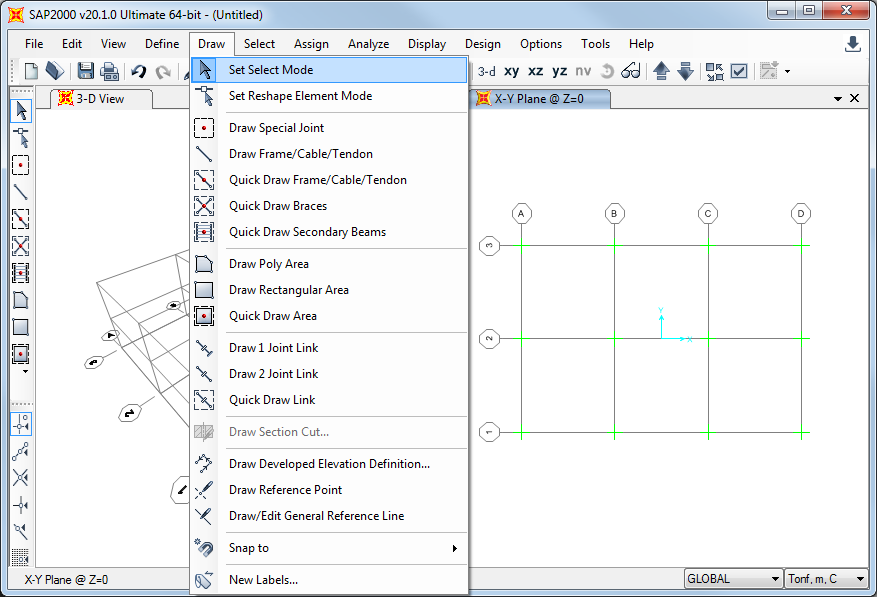
\includegraphics[width=1\textwidth]{metodologia/sap2000_draw.png}
%     \caption{Menú de SAP2000\textsuperscript{\textregistered} que permite ingresar diferentes tipos de elementos.}
%     \label{fig:sap200_draw}
% \end{figure}

% Una vez el usuario haya agregado los diferentes elementos de la estructura puede modificar sus condiciones de apoyo, las cargas, entre otros, mediante el uso de menús, de manera que el modelo esté listo para que el programa ejecute el análisis correspondiente. En la figura \ref{fig:sap2000_model} se presenta el modelo de una estructura terminado.
% \begin{figure}[ht]
%     \centering
%     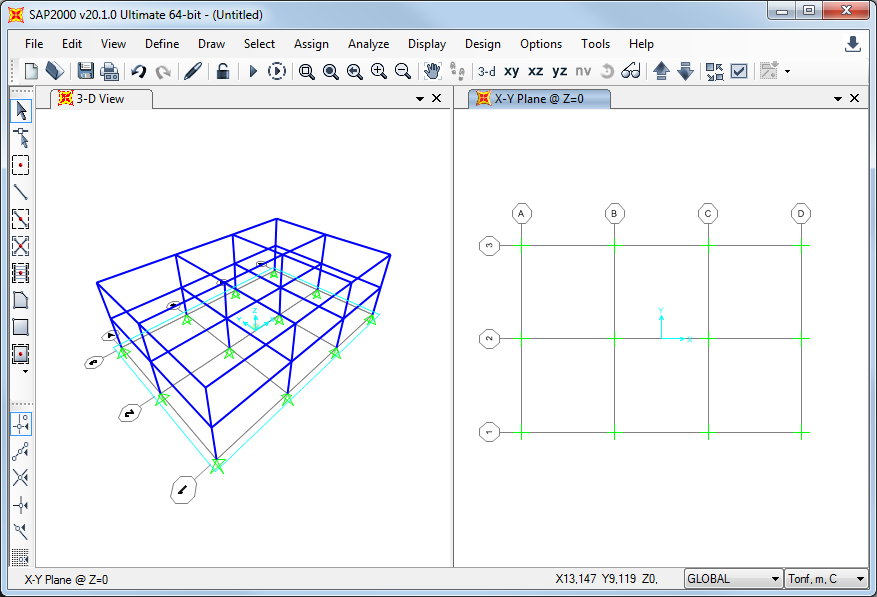
\includegraphics[width=1\textwidth]{metodologia/sap2000_model.png}
%     \caption{Modelo de una estructura en  SAP2000\textsuperscript{\textregistered}.}
%     \label{fig:sap2000_model}
% \end{figure}

% Una vez se han surtido los pasos anteriores, el usuario puede correr el análisis para obtener los resultados del mismo. El usuario puede visualizar los resultados en el entorno virtual, como se muestra en la figura \ref{fig:sap2000_deformed}, o mediante tablas.
% \begin{figure}[ht]
%     \centering
%     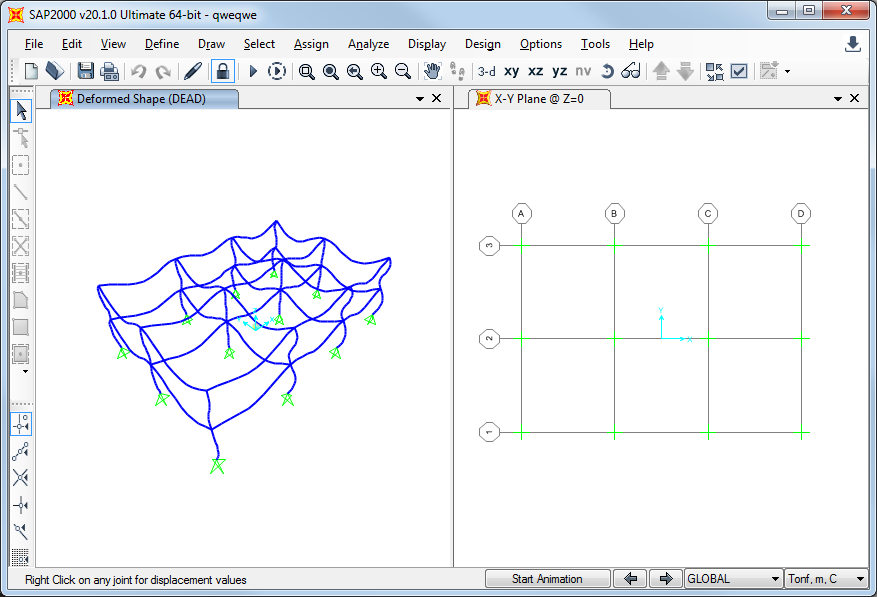
\includegraphics[width=1\textwidth]{metodologia/sap2000_deformed.png}
%     \caption{Deformación de la estructura después del análisis de SAP2000\textsuperscript{\textregistered}.}
%     \label{fig:sap2000_deformed}
% \end{figure}

% Así como el programa SAP2000\textsuperscript{\textregistered}, los otros programas comerciales, como ETABS \textsuperscript{\textregistered}, CSIBridge\textsuperscript{\textregistered}, midas\textsuperscript{\textregistered}, entre otros, cuentan con herramientas similares para que el usuario pueda analizar modelos de estructuras.

% \section{Revisión de los programas a código abierto}
% Existen gran variedad de programas a código abierto. Entre los programas que más se han estudiado para este trabajo se encuentra \textit{ANALEST}. \\

% El programa \textit{ANALEST} comprende una serie de subprogramas cuyo objeto es servir de ayuda en el análisis y diseño de estructuras. El programa está programado en \texttt{BASIC} y su característica principal es analizar 
% \begin{inparaenum}[$ (1) $]
%     \item vigas continúas, 
%     \item armaduras planas, 
%     \item armaduras en el espacio, 
%     \item pórticos planos, 
%     \item pórticos en el espacio, 
%     \item parrillas planas.
% \end{inparaenum}

% Para usar los subprogramas, se debe
% \begin{inparaenum}[$ (1) $]
%     \item introducir los datos del modelo de la estructura, revisarlos y guardarlos, 
%     \item introducir los datos de carga, revisarlos y guardarlos, 
%     \item ejecutar el análisis, guardar los resultados y presentarlos
% \end{inparaenum}

% Ademas, los subprogamas de vigas y armaduras permiten encontrar la envolvente de momentos en los apoyos y de fuerzas axiales, respectivamente, como paso preliminar para el diseño de los miembros. \\

% Guardar los datos estructurales y los datos de carga es muy útil en aquellos casos en que conviene modificar las dimensiones de los elementos con base en los resultados del primer análisis. Por otra parte, guardar los resultados facilita el estudio de las combinaciones de carga disminuyendo por una parte los datos requeridos y por otra el tiempo de ejecución, ya que se aprovecha el principio de superposición. Adicionalmente, guardar dichos resultados facilita el enlace de los subprogramas con programas de diseño, bien sean adquiridos o desarrollados por el usuario. \\

% \section{Identificación de los elementos a programar}

% De la revisión de los diferentes programas comerciales se dedujo que el programa StressUN debía dividirse en tres partes y que tenían que trabajar en conjunto. Dichas partes son: \textit{preproceso}, \textit{proceso} y \textit{posproceso}. \\

% El preproceso consiste en la adquisición de todos los datos relevantes del modelo de la estructura a analizar. El proceso realiza el tratamiento de los datos del modelo, mientras que el posproceso presenta los resultados del análisis del modelo. \\

% Tanto el preproceso como el posproceso necesitan de un ambiente gráfico, mientras que el proceso necesita de las rutinas propias del análisis matricial. \\

% \section{Selección de las herramientas de programación}
% Los dos grandes problemas a solucionar consistieron en desarrollar el ambiente gráfico, el cual se compone de menús y un entorno virtual tridimensional, y el núcleo de StressUN. Para esto, se consultó las diferentes herramientas de programación disponibles, donde se decidió utilizar la librería \textit{frames}, la cual está programada en el \textit{Java}, y el conjuto de librerías \textit{Scipy}, la cual está programada en \textit{Python}.\\

% La librería frames consiste en un conjunto de herramientas para crear un entorno virtual bidimensional o tridimensional interactivo. Dicha librería trabaja como una extensión de la librería \textit{processing}, la cual también está programada en Java. \\

% La librería processing es un conjunto de herramientas dirigida a solucionar los problemas relacionados con la computación gráfica, permitiendo a los desarrolladores desde crear imágenes hasta entornos virtuales tridimensionales. \\

% Por otro lado, el conjunto de librerías Scipy consiste en herramientas para solucionar problemas relacionados algebra matricial. Dicho conjunto de librerías está conformado por \textit{Numpy}, \textit{Scipy}, \textit{matplotlib}, entre otros. La librería Numpy provee arreglos multidimensionales y operaciones entre ellos. La librería \textit{Scipy} trata problemas del algebra matricial, como son la solución de sistemas de ecuaciones líneales, mientras que matplotlib permite generar diferentes tipos de gráficos. \\

% \section{Desarrollo del programa de computador}

% Una vez se identificaron los diferentes elementos necesarios con los que debía contar el programa de computador y se escogieron las herramientas de trabajo, se realizó una revisión bibliográfica de la formulación matemática de los métodos matriciales aplicados al análisis estructural, enfocada al análisis de estructuras tridimensionales de respuesta lineal. Adicionalmente, se realizó una revisión a la documentación de la librería frames.\\

% De dicho ejercicio se identificaron los datos de entrada que el usuario necesita definir y los datos de salida que espera obtener
% \begin{itemize}
%     \item \textit{Preproceso}
%     \begin{itemize}
%         \item Definición de los materiales.
%         \item Definición de las secciones transversales.
%         \item Definición de los nudos.
%         \item Definición de los elementos.
%         \item Definición de las condiciones de apoyo.
%         \item Definición de los casos de carga.
%         \item Definición de las combinaciones de carga.
%         \item Definición de las patrones de carga
%     \end{itemize}
%     \item \textit{Posproceso}
%     \begin{itemize}
%         \item Visualización de los desplazamientos en los nudos.
%         \item Visualización de las reacciones.
%         \item Visualización de las fuerzas internas.
%     \end{itemize}
    
% \end{itemize}

%  \textit{StressUN} se desarrolló usando el paradigma de \textit{programación orientada a objetos}, \textit{OOP} (de sus siglas en inglés \textit{object-oriented programming}), y en forma modular, de manera que el \textit{preproceso} y el \textit{posproceso} son independientes del \textit{proceso}.\\

% A medida que se definieron los diferentes elementos a tener en cuenta, se fueron programando. Es decir, se desarrollaron las clases \textit{primitivas} del programa, las cuales representan la abstracción de los elementos de las entidades más sencillas del problema, las cuales consisten en las clases
% \begin{itemize}
%     \item \textit{Material}.
%     \item \textit{Section}.
%     \item \textit{Node}.
%     \item \textit{Frame}.
%     \item \textit{Support}.
%     \item \textit{PointLoad}.
%     \item \textit{LoadPattern}.
%     \item \textit{Displacement}.
% \end{itemize}

% Las clases anteriormente listadas, tienen su representación tanto en el preproceso y posproceso, como en el proceso. Es decir, en el preproceso y posproceso dichas clases tienen su representación gráfica, mientras que en el proceso, éstos tienen su representación matemática. Sin embargo, dichas clases son separadas unas de las otras, de manera que se asegure que el preproceso y posproceso son independientes del proceso.

% Una vez programados las entidades más básicas del programa, se procedió a crear la clase \textit{Structure}, la cual se encarga de administrar otros objetos. Dicho paradigma de programación se conoce como \textit{composición}. Los objetos que contiene la clase \textit{Structure} son

% \begin{itemize}
%     \item \textit{Materials}.
%     \item \textit{Sections}.
%     \item \textit{Nodes}.
%     \item \textit{Frames}.
%     \item \textit{Supports}.
%     \item \textit{LoadPatterns}.
% \end{itemize}

% Cada una de las anteriores clases es la interfaz entre el programa y el usuario, donde este último podrá agregar nuevos materiales, secciones, nudos, elementos tipo pórtico, condiciones de apoyo y condiciones de carga. Dichas clases componen el \textit{núcleo} del programa.\\

% El proceso anteriormente descrito se desarrolló bajo los diferentes mecanismos que provee la programación orientada objeto, los cuales son encapsulación, herencia y sobre carga. Estas herramientas, bien aplicadas, permiten la reutilización del código y el mantenimiento del mismo. Así mismo, se utilizó la herramienta de \textit{Git}, la cual es un sistema de control de versiones, la cual permite llevar el control absoluto durante el proceso de desarrollo del código.\\

% \section{Verificación del programa}

% Una vez se llegó a una versión estable del programa, este se puso a prueba mediante la solución de diferentes problemas que aparecen en la bibliografía, donde se comparó la respuesta obtenida con la presentada. Así mismo, se comparó el desempeño del programa frente a otros programas, tanto comerciales como académicos, en cuanto a la facilidad de uso como al tiempo de computo. \\